%%%%%%%%%%%%%%%%%%%%%%%%%%%%%%%%%%%%%%%%%
% Short Sectioned Assignment
% LaTeX Template
% Version 1.0 (5/5/12)
%
% This template has been downloaded from:
% http://www.LaTeXTemplates.com
%
% Original author:
% Frits Wenneker (http://www.howtotex.com)
%
% License:
% CC BY-NC-SA 3.0 (http://creativecommons.org/licenses/by-nc-sa/3.0/)
%
%%%%%%%%%%%%%%%%%%%%%%%%%%%%%%%%%%%%%%%%%

%----------------------------------------------------------------------------------------
%	PACKAGES AND OTHER DOCUMENT CONFIGURATIONS
%----------------------------------------------------------------------------------------

\documentclass[paper=a4, fontsize=11pt]{scrartcl} % A4 paper and 11pt font size

\usepackage[T1]{fontenc} % Use 8-bit encoding that has 256 glyphs
\usepackage{fourier} % Use the Adobe Utopia font for the document - comment this line to return to the LaTeX default
\usepackage[french]{babel} % English language/hyphenation
\usepackage{amsmath,amsfonts,amsthm} % Math packages

\usepackage{lipsum} % Used for inserting dummy 'Lorem ipsum' text into the template

\usepackage{sectsty} % Allows customizing section commands
\allsectionsfont{\centering \normalfont\scshape} % Make all sections centered, the default font and small caps

\usepackage{graphicx}
\graphicspath{ {images/} }
\usepackage{listings}
\lstset{
  basicstyle=\small,
  columns=fullflexible,
  frame=single,
  breaklines=true
}

\usepackage[utf8]{inputenc}

\usepackage{fancyhdr} % Custom headers and footers
\pagestyle{fancyplain} % Makes all pages in the document conform to the custom headers and footers
\fancyhead{} % No page header - if you want one, create it in the same way as the footers below
\fancyfoot[L]{} % Empty left footer
\fancyfoot[C]{} % Empty center footer
\fancyfoot[R]{\thepage} % Page numbering for right footer
\renewcommand{\headrulewidth}{0pt} % Remove header underlines
\renewcommand{\footrulewidth}{0pt} % Remove footer underlines
\setlength{\headheight}{13.6pt} % Customize the height of the header

\numberwithin{equation}{section} % Number equations within sections (i.e. 1.1, 1.2, 2.1, 2.2 instead of 1, 2, 3, 4)
\numberwithin{figure}{section} % Number figures within sections (i.e. 1.1, 1.2, 2.1, 2.2 instead of 1, 2, 3, 4)
\numberwithin{table}{section} % Number tables within sections (i.e. 1.1, 1.2, 2.1, 2.2 instead of 1, 2, 3, 4)

\setlength\parindent{0pt} % Removes all indentation from paragraphs - comment this line for an assignment with lots of text

%----------------------------------------------------------------------------------------
%	TITLE SECTION
%----------------------------------------------------------------------------------------

\newcommand{\horrule}[1]{\rule{\linewidth}{#1}} % Create horizontal rule command with 1 argument of height

\title{	
\normalfont \normalsize 
\textsc{HEIG-VD, MAC} \\ [25pt] % Your university, school and/or department name(s)
\horrule{0.5pt} \\[0.4cm] % Thin top horizontal rule
\huge Lab02 Transactions \\ % The assignment title
\horrule{2pt} \\[0.5cm] % Thick bottom horizontal rule
}

\author{Lawrence Stalder, Valentin Finini} % Your name

\date{\normalsize\today} % Today's date or a custom date

\begin{document}

\maketitle % Print the title

%----------------------------------------------------------------------------------------
%	Presentation
%----------------------------------------------------------------------------------------

\section{Modèles}

\subsection{Modèle Relationnel}

Le modèle relationnel pour la base de \textit{Transactions} est représenté dans la fig \ref{fig:rela}. A noter qu'il est tout a fait normal que la table \textit{journal} ne soit pas reliée au reste de la base de donnée. Car si quelque chose venait à être ajouté/supprimé, la table \textit{journal} ne devrait pas être affectée.

\begin{figure}[h]
  \centering
  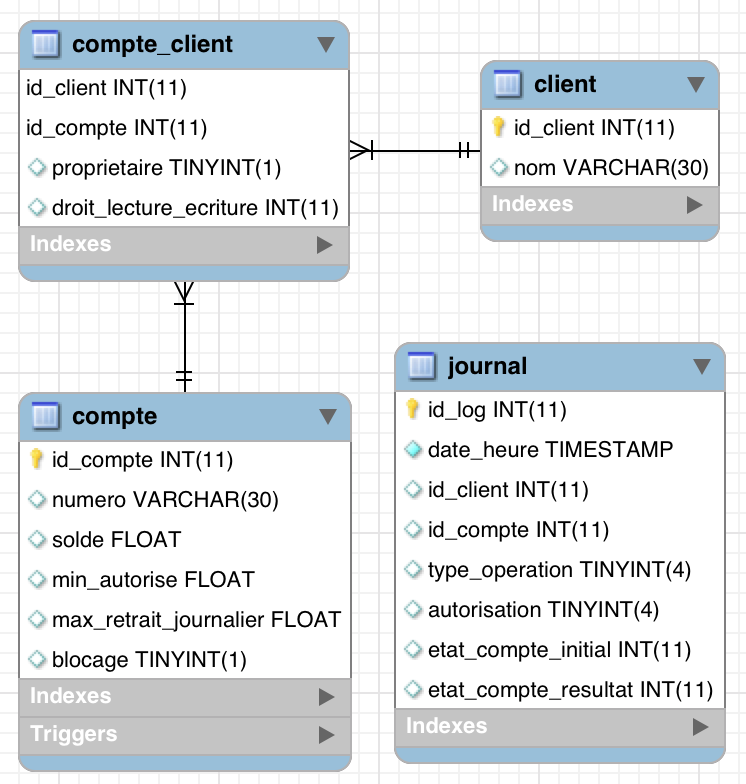
\includegraphics[height=200px]{relationnel.png}
  \caption{Modèle relationnel de la base de données \textit{Transactions}}
  \label{fig:rela}
\end{figure}

%------------------------------------------------

\subsection{Modèle Entités-Associations}

La plus part des contraintes de fonctionnements devraient être traitées par des triggers. Voilà un détail pour chaque contraite.

\begin{figure}[h]
  \centering
  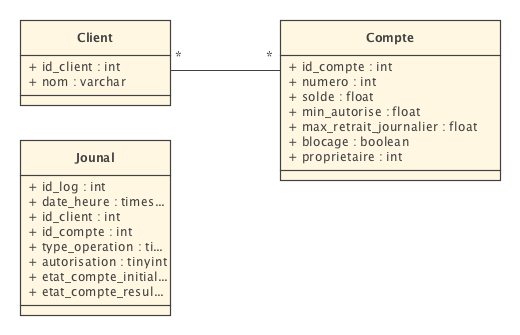
\includegraphics[height=200px]{entites.png}
  \caption{Modèle entités associations de la base de données \textit{Transactions}}
  \label{fig:entites}
\end{figure}

\begin{enumerate}
	\item Procédure stockée pour effectuer un retrait
	\item Ajout dans la procédure citée ci-dessus, avec lecture de la table \textit{journal}
	\item Ajout d'un trigger à la création d'un compte, qui ajoute une entrée dans \textit{compte client} avec l'entrée proprietaire à \textit{true}
	\item Trigger crée pour l'admin
	\item Ajout d'un trigger avant la suppression d'un client, vérification dans \textit{compte client}
	\item Ajout d'un trigger avant une insertion dans \textit{compte client}, vérification si le client n'est pas déjà associé au compte
\end{enumerate}

%------------------------------------------------

\subsection{Création des utilisateurs}

Afin de créer les utilisateurs, nous avons utilisé les requêtes MYSQL suivantes. 
\begin{lstlisting}
CREATE USER IF NOT EXISTS 'u1'@'%' IDENTIFIED BY 'u1';
CREATE USER IF NOT EXISTS 'u2'@'%' IDENTIFIED BY 'u2';
CREATE USER IF NOT EXISTS 'u3'@'%' IDENTIFIED BY 'u3';

INSERT into client(nom) VALUES ('u1');
INSERT into client(nom) VALUES ('u2');
INSERT into client(nom) VALUES ('u3');
\end{lstlisting}

Ensuite afin de spécifier les droits que ces utilisateurs ont il suffi de leur assigner des permissions sur les procédures stockées.
\begin{lstlisting}
GRANT EXECUTE ON PROCEDURE transactions.lire_compte TO 'u1'@'%';
GRANT EXECUTE ON PROCEDURE transactions.depot_compte TO 'u1'@'%';
GRANT EXECUTE ON PROCEDURE transactions.lire_compte TO 'u2'@'%';
GRANT EXECUTE ON PROCEDURE transactions.depot_compte TO 'u2'@'%';
GRANT EXECUTE ON PROCEDURE transactions.lire_compte TO 'u3'@'%';
GRANT EXECUTE ON PROCEDURE transactions.depot_compte TO 'u3'@'%';
\end{lstlisting}

L'administateur a tous les droits.
\begin{lstlisting}
CREATE USER IF NOT EXISTS 'admin1234'@'localhost' IDENTIFIED BY 'nimda';
GRANT ALL PRIVILEGES ON *.* TO 'admin'@'localhost';
\end{lstlisting}

%------------------------------------------------

\subsection{Trigger et procédures}
\subsubsection{Suppresion d'un compte par l'admin}

Il nous est demandé de réaliser un trigger pour l'administrateur afin qu'il soit impossible de supprimer un compte si son solde n'est pas nul. Le trigger est en soit assez simple, il envoie simplement une erreur si l'operation n'est pas possible car le solde est superieur à 0.


\begin{lstlisting}
DELIMITER //
CREATE TRIGGER suppression_compte
BEFORE DELETE ON compte FOR EACH ROW
BEGIN
	IF (solde > 0.0) THEN
		SIGNAL SQLSTATE '45000' SET MESSAGE_TEXT 
			= 'PAS POSSIBLE, SOLDE SUPERIEUR A 0!';
	else
		INSERT into journal(date_heure, id_compte, 
			type_operation, autorisation)
        VALUES (NOW(), OLD.id_compte, 2, 5);
	END IF;
END //
DELIMITER ;
\end{lstlisting}


\subsubsection{Lecture du solde d'un compte}
Pour la lecture d'un compte nous avons une procédure qui accepte deux paramètres, le premier désigne le numero de compte, le deuxième est une variable de retour dans laquelle le resultat sera assigné.

En ce qui concerne l'implémentation, nous avons choisi de garder des opérations très simples, ce qui demande un certain nombre de déclarations de variables. Il nous a semblé plus clair de ne pas trop imbriquer d'appels, cela aurait rendu la lecture bien plus compliquée..

Notons que \textit{SUBSTRING INDEX} permet de récuperer le nom de l'utilisateur appelant la procédure. La procédure gère également l'ajout de l'entrée dans le \textit{journal}. Elle vérifie également que l'appelant a au minimum les droits de lecture sur le compte spécifié.

\begin{lstlisting}
DELIMITER //
DROP PROCEDURE IF EXISTS lire_compte //
CREATE PROCEDURE lire_compte(in numero_compte int(11), out etat float)
BEGIN
	
    DECLARE username varchar(30);
    DECLARE id_username int(11);
	DECLARE id_compte_depot int(11);
    DECLARE droits int(11);
    
    SELECT SUBSTRING_INDEX(user(), '@', 1) into username;
    
    SELECT id_client into id_username
    FROM client 
		WHERE client.nom = username;
        
	SELECT id_compte into id_compte_depot
    FROM compte
		WHERE numero_compte = numero;
        
	SELECT droit_lecture_ecriture into droits
    FROM compte_client
		WHERE id_compte = id_compte_depot 
			AND id_client = id_username;
			 
    IF (droits >= 1) THEN
		SELECT solde into etat
		FROM compte 
			WHERE id_compte = id_compte_depot;
		
        INSERT into journal(date_heure, id_client,
        	id_compte, type_operation, autorisation)
			VALUES(NOW(), id_username, id_compte_depot, 0, 0);
	ELSE
		INSERT into journal(date_heure, id_client,
			id_compte, type_operation, autorisation)
			VALUES(NOW(), id_username, id_compte_depot, 0, 3);
            
		SIGNAL SQLSTATE '45000' SET MESSAGE_TEXT 
			= 'PAS POSSIBLE, PAS LES DROITS!';
	END IF;
END //
DELIMITER ;
\end{lstlisting}


\subsubsection{Dépot sur un compte}
Voici la procédure pour effectuer un dépot sur un compte. Cette dernière accepte deux paramètres, le premier est le numéro de compte à créditer, le deuxième est le montant. La procédure vérifie que l'utilisateur ait les droits d'écriture sur le compte. Comme pour la lecture de compte nous avons opté pour écriture simple et lisible, ce qui se traduit par la déclaration de beaucoup de variables. Le journal est mis à jour avec le résultat de l'opération, si l'écriture à lieu ou si les permissions ne sont pas réspectées.

\begin{lstlisting}
DELIMITER //
DROP PROCEDURE IF EXISTS depot_compte //
CREATE PROCEDURE depot_compte(in numero_compte int(11), in depot float)
BEGIN
	
    DECLARE username varchar(30);
    DECLARE id_username int(11);
    DECLARE id_compte_depot int(11);
    DECLARE droits int(11);
    DECLARE solde_curr float;
    
    SELECT SUBSTRING_INDEX(user(), '@', 1) into username;
    
    SELECT id_client into id_username
    FROM client 
		WHERE client.nom = username;
        
	SELECT id_compte into id_compte_depot
    FROM compte
		WHERE numero_compte = numero;

	SELECT droit_lecture_ecriture into droits
    FROM compte_client
		WHERE id_username = id_client 
			AND id_compte = id_compte_depot;
     
	SELECT solde into solde_curr
	FROM compte
		WHERE id_compte = id_compte_depot;
             
    IF (droits >= 2.0) THEN
		
        INSERT into journal(date_heure, id_client,
        	id_compte, type_operation, 
        	autorisation, etat_compte_initial, 
        	etat_compte_resultat)
			VALUES(NOW(), id_username, id_compte_depot, 
				1, 0, solde_curr, solde_curr + depot);
            
		UPDATE compte
			SET solde = depot + solde
			WHERE id_compte = id_compte_depot;

	ELSE
		INSERT into journal(date_heure, id_client, 
			id_compte, type_operation,
			autorisation, etat_compte_initial, 
			etat_compte_resultat)
			VALUES(NOW(), id_username, id_compte_depot, 
				1, 4, solde_curr, solde_curr);
            
		SIGNAL SQLSTATE '45000' SET MESSAGE_TEXT 
			= 'PAS POSSIBLE, PAS LES DROITS!';
	END IF;
END //
DELIMITER ;
\end{lstlisting}

%----------------------------------------------------------------------------------------
%	Testing
%----------------------------------------------------------------------------------------
\newpage
\section{Tests d'executions}
Dans un premier temps il s'agit d'executer le script sur fichier \textit{transactions.sql} voici le resultat de l'execution.

\begin{figure}[h]
  \centering
  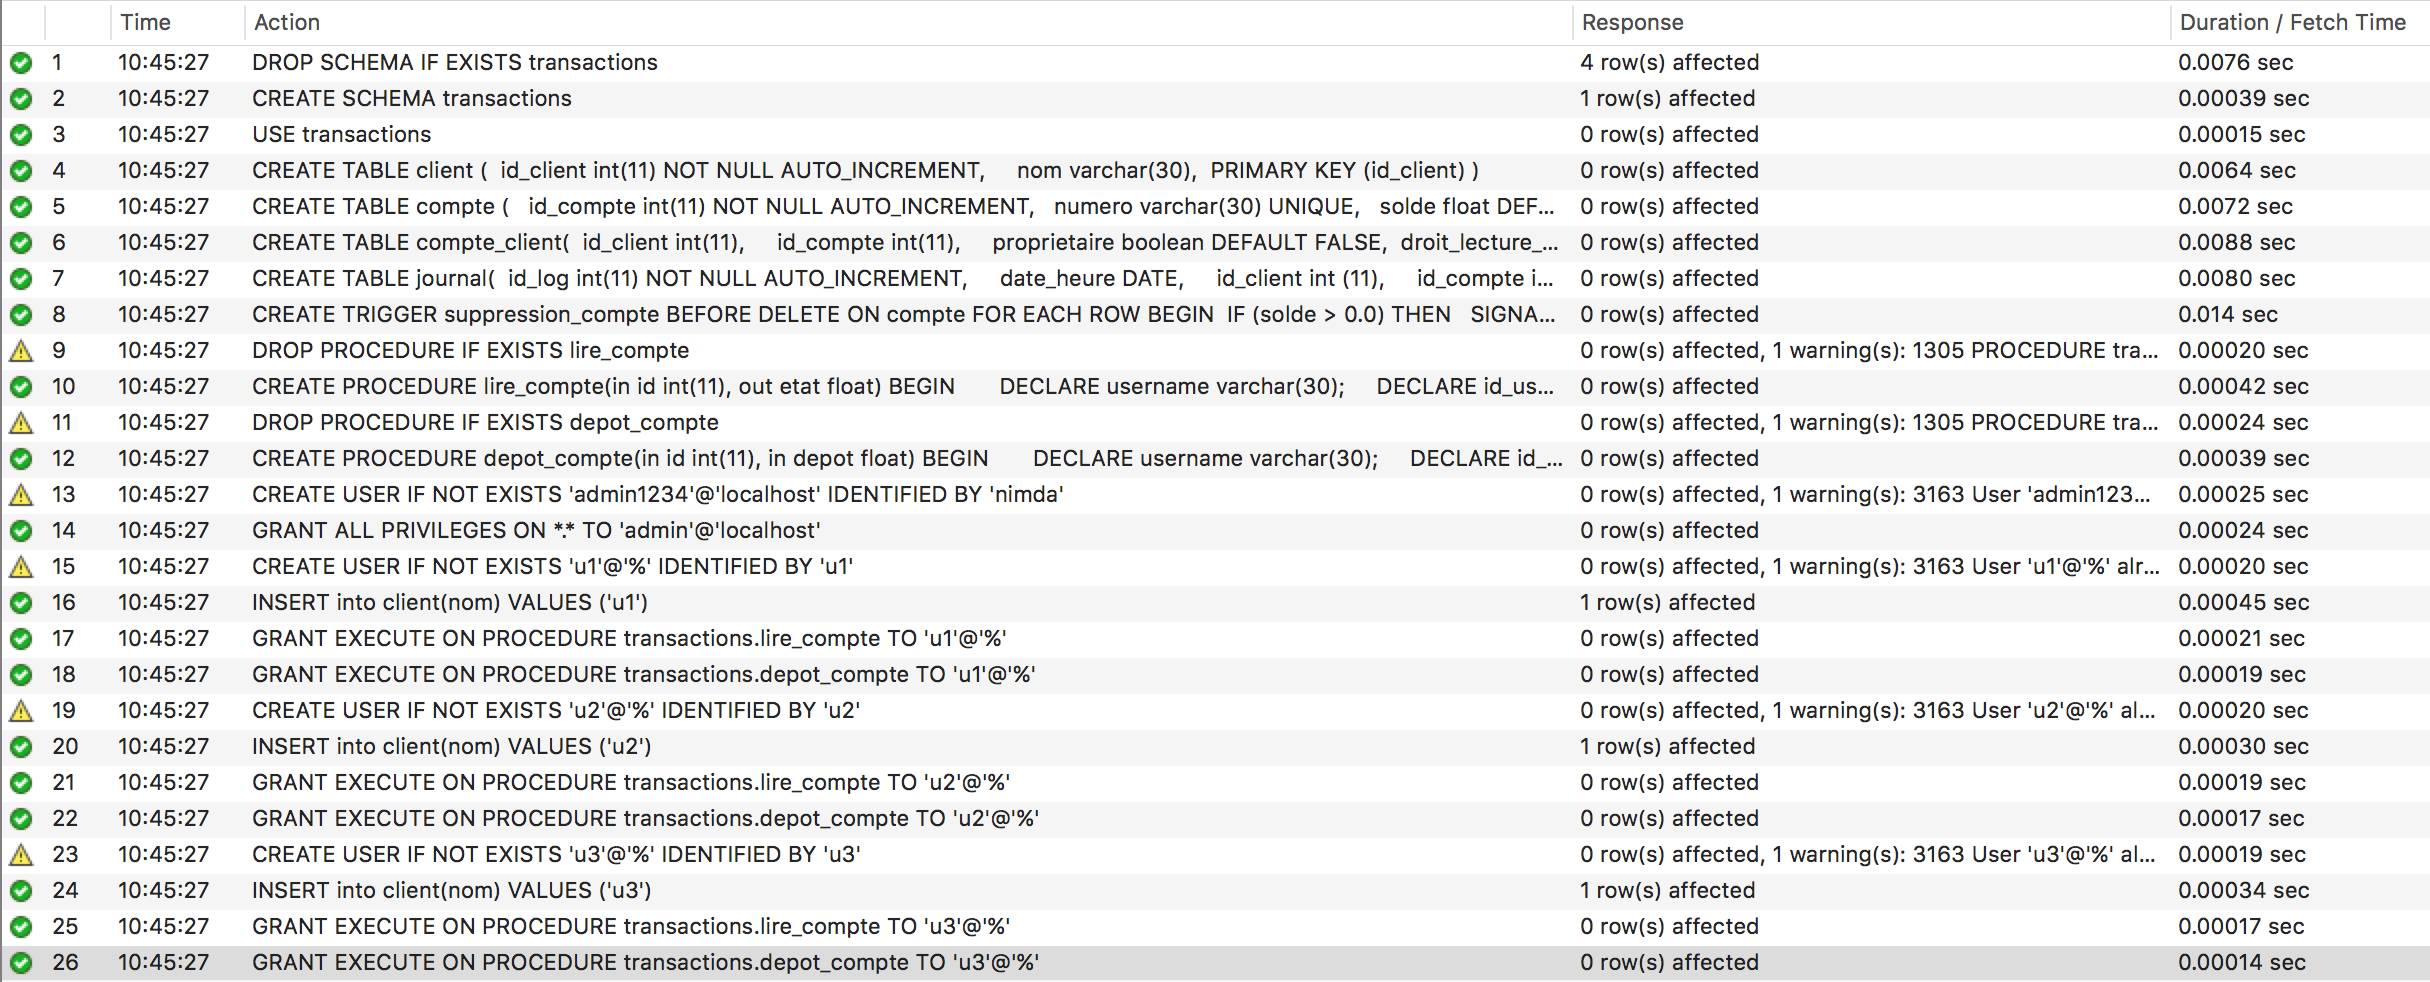
\includegraphics[width=\textwidth]{sqlCreate.png}
  \caption{Execution de la création de la base de donnée \textit{Transactions}}
  \label{fig:sql}
\end{figure}

Ensuite voici les tests que nous effectuons pour vérifier le bon fonctionnement de nos contraintes. L'utilisateur \textit{u1} à les droits d'écritures sur le compte 1010, les droits de lecture uniquement sur le compte 2020 et n'a aucun droits sur le compte 3030. 

La dernière ligne sert à vérifier que l'utilisateur ne peut pas modifier directement les tables de la base de donnée, seul l'administrateur le peut.

\begin{lstlisting}
call transactions.lire_compte(1010, @solde);
SELECT concat("Solde compte 1: ", @solde);

call transactions.lire_compte(2020, @solde);
SELECT concat("Solde compte 2: ", @solde);

call transactions.lire_compte(3030, @solde);

call transactions.depot_compte(1010, 1000);

call transactions.depot_compte(2020, 2500);

UPDATE compte SET solde = 99999
	WHERE id_compte = 1010;
\end{lstlisting}

La figure suivante illustre les résultats d'exection. 

\begin{figure}[h]
  \centering
  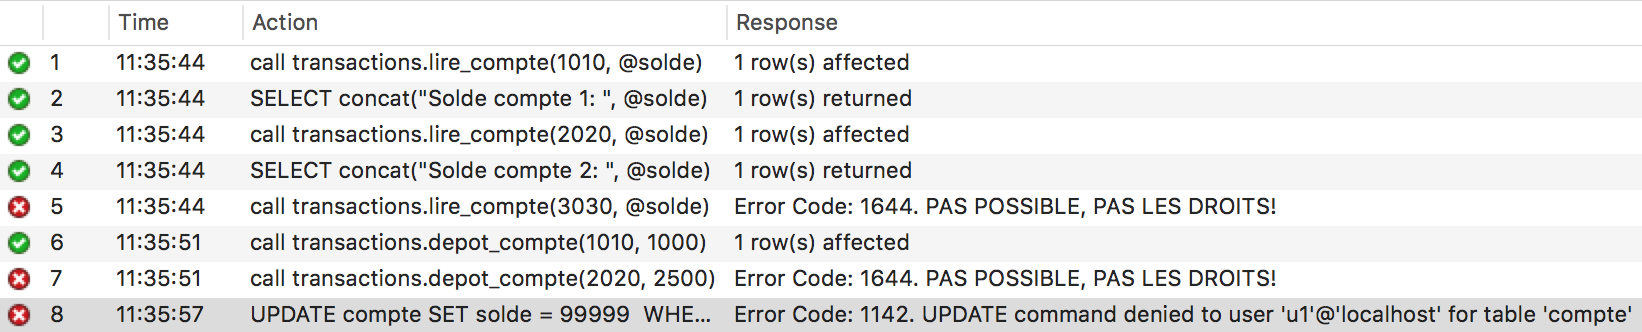
\includegraphics[width=\textwidth]{tests.png}
  \caption{Résultats de l'executions des tests pour l'utilisateur \textit{u1}}
  \label{fig:test}
\end{figure}


%----------------------------------------------------------------------------------------
%	Files
%----------------------------------------------------------------------------------------
\newpage
\section{Fichiers SQL}
Ci dessous, en annexe, les fichiers SQL de la base de donnée ainsi que les tests.

\lstinputlisting{transactions.sql}
\lstinputlisting{tests.sql}


\end{document}